\documentclass[11pt, oneside]{article}  % need to compile twice
\usepackage{amsmath, textcomp, amssymb, geometry, graphicx, enumerate, ctex, fancyhdr, float}
\usepackage[colorlinks, linkcolor=black]{hyperref}
\usepackage{multirow}
\usepackage[normalem]{ulem}
\usepackage{subcaption}
\useunder{\uline}{\ul}{}

\usepackage{listings}		% 为了避免与页眉的兼容问题可将listings放入table环境中
\lstset{
    basicstyle          =   \sffamily,          % 基本代码风格
    keywordstyle        =   \bfseries,          % 关键字风格
    commentstyle        =   \rmfamily\itshape,  % 注释的风格, 斜体
    stringstyle         =   \ttfamily,  % 字符串风格
    flexiblecolumns,                % 别问为什么, 加上这个
    numbers             =   left,   % 行号的位置在左边
    showspaces          =   false,  % 是否显示空格, 显示了有点乱, 所以不现实了
    numberstyle         =   \zihao{-5}\ttfamily,    % 行号的样式, 小五号, tt等宽字体
    showstringspaces    =   false,
    captionpos          =   t,      % 这段代码的名字所呈现的位置, t指的是top上面
    frame               =   lrtb,   % 显示边框
}

\geometry{left=2.54cm, right=2.54cm, top=3.18cm, bottom=3.18cm}

\def\Name{杨豪\space}  % Your name
\def\SID{2206213297}  % Your student ID number

% need to be confirmed before each time writing and committing 
\def\Homework{3} % Number of Homework
\def\Session{2022-Fall}
\def\CourseCodeName{SOFT410911: Software Quality Assurance}
\def\simCourseName{SQA}

\title{\vspace{-4cm}\CourseCodeName \space
        \Session \protect\\  Homework-\textbf{\Homework} Solutions}
\author{软件2101 \Name \space 学号: \SID}
\date{\today}

\markright{\simCourseName\ \space \Session\  HW-\Homework\ \Name}

\begin{document}

\maketitle

\textbf{Honor Code: I promise that I finished the homework solutions on my own without copying other people's work.}

\section*{Equivalence partitioning}

\subsection*{1. Topic: from Idea to Reality}

In HW-2, I chose creation account as topic of my test list and divided them into distinct kinds. 
In this homework, I will reuse this idea but in a more real circumstance ——~creating \textbf{QQ} account. 
(\url{https://zc.qq.com/chs/index.html})

\subsection*{2. Observation for Input Partition}

\begin{figure}[H]
    \centering
    
\includegraphics[width = 0.5\textwidth]{pic/3.0.png}
\end{figure}

There are several input fields: 

\begin{enumerate}
    \item \textbf{Nickname}. After several tests, it seems that there is no limitation for nickname except 
        \textbf{cannot be empty}. 
    \item \textbf{Password}. 3 limitation of Password as below.
        \begin{figure}[H]
            \centering
            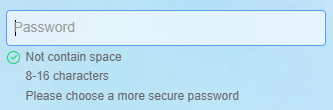
\includegraphics[width = 0.5\textwidth]{pic/3.1.png}
        \end{figure}
    \item \textbf{Tel}. After pressing the send button of Code, it will examine whether the phone number is valid.
        \begin{itemize}
            \item \textbf{Country of Tel}. 
        \end{itemize}
    \item \textbf{Code}. Input should be identified with the sent code.
        \begin{itemize}
            \item \textbf{Security Verify}. Drag a icon to given place. 
                \begin{figure}[H]
                    \centering
                    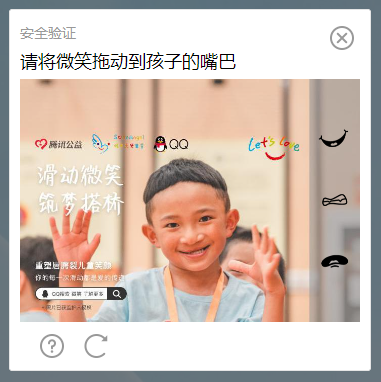
\includegraphics[width = 0.5\textwidth]{pic/3.2.png}
                \end{figure}
        \end{itemize}
    \item \textbf{Service Agreement}. Should be accepted. 
\end{enumerate}


\subsection*{3. Equivalence Partitioning Test List}

\begin{table}[H]
    \centering
    \begin{tabular}{|c|c|c|c|c|}
        \hline
                                   & \textbf{valid partition}      & \textbf{invalid partition}      \\ \hline
        \textbf{Nickname}          & not empty                     & empty       \\ \hline
        \textbf{Password Length}   & 8-16                          & >8, <16    \\ \hline
        \textbf{Password char}     & not contain space             & contain space      \\ \hline
        \textbf{Password Security} & secure (as stipulated inside) & not secure enough       \\ \hline
        \textbf{Tel}               & valid number after check      & invalid number  \\ \hline
        \textbf{Agreement}         & Accept                        & Not Accept    \\ \hline
        \textbf{Code}              & same as a random number       & others \\ \hline
        \textbf{Security Verify}   & close to certain space        & far  \\ \hline
    \end{tabular}
\end{table}

\subsection*{4. Exact Test \& Test Results}

\begin{figure}[H]
    \centering
	\begin{subfigure}{0.4\linewidth}
		
\includegraphics[width=1\linewidth]{./pic/3.3.1.png}
        \caption{valid test: 啊。     1?}
	\end{subfigure}
    \begin{subfigure}{0.4\linewidth}
		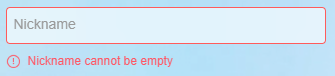
\includegraphics[width=1\linewidth]{./pic/3.3.2.png}
        \caption{invalid test: (empty)}
	\end{subfigure}
    \caption{test for Nickname}
\end{figure}

\begin{figure}[H]
    \centering
    \begin{subfigure}{0.4\linewidth}
		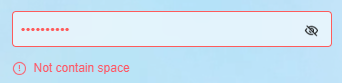
\includegraphics[width=1\linewidth]{./pic/3.3.3.png}
        \caption{invalid space test: 12345678 9}
	\end{subfigure}
    \begin{subfigure}{0.4\linewidth}
		
\includegraphics[width=1\linewidth]{./pic/3.3.4.png}
        \caption{invalid length test: 1234}
	\end{subfigure}
    \begin{subfigure}{0.4\linewidth}
		
\includegraphics[width=1\linewidth]{./pic/3.4.4.png}
        \caption{invalid security test: 12121212}
	\end{subfigure}
    \begin{subfigure}{0.4\linewidth}
		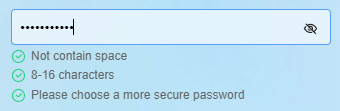
\includegraphics[width=1\linewidth]{./pic/3.4.3.png}
        \caption{valid test: 12121212pp}
	\end{subfigure}
    \caption{test for Password\\(another invalid length test: but input is not allowed for more than 16 characters)}
\end{figure}

\begin{figure}[H]
    \centering
	\begin{subfigure}{0.4\linewidth}
		
\includegraphics[width=1\linewidth]{./pic/3.3.9.png}
        \caption{valid test: 183941*****(my own Tel)}
	\end{subfigure}
    \begin{subfigure}{0.4\linewidth}
		
\includegraphics[width=1\linewidth]{./pic/3.3.6.png}
        \caption{invalid test: 12345678909}
	\end{subfigure}
    \caption{test for Tel}
\end{figure}

\begin{figure}[H]
    \centering
	\begin{subfigure}{0.4\linewidth}
		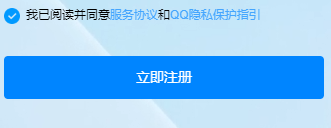
\includegraphics[width=1\linewidth]{./pic/3.4.2.png}
        \caption{valid test: (accept)}
	\end{subfigure}
    \begin{subfigure}{0.4\linewidth}
		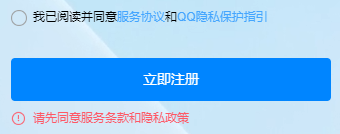
\includegraphics[width=1\linewidth]{./pic/3.4.1.png}
        \caption{invalid test: (not accept)}
	\end{subfigure}
    \caption{test for Agreement}
\end{figure}

\begin{figure}[H]
    \centering
    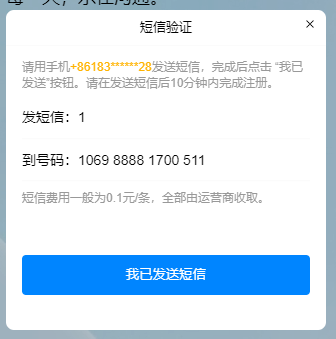
\includegraphics[width=0.5\textwidth]{pic/3.3.8.png}
    \caption{test for Code \\ Here QQ detects that my Tel registered an account, \\ so it asks me to send a code to it, \\which is definitely secure.}
\end{figure}

\begin{figure}[H]
    \centering
	\begin{subfigure}{0.4\linewidth}
		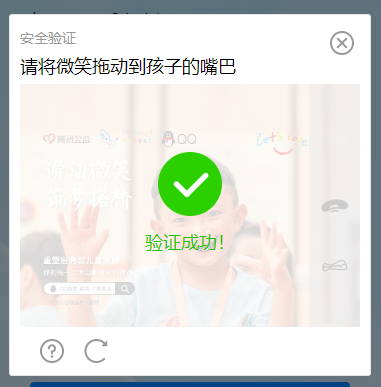
\includegraphics[width=1\linewidth]{./pic/3.3.7.png}
        \caption{valid test: (passed)}
	\end{subfigure}
    \begin{subfigure}{0.4\linewidth}
		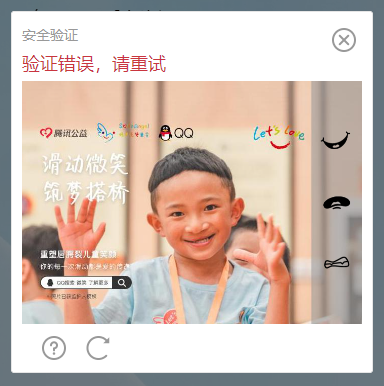
\includegraphics[width=1\linewidth]{./pic/3.3.5.png}
        \caption{invalid test: (far)}
	\end{subfigure}
    \caption{test for Verification}
\end{figure}

\subsection*{5. Summary}
After comparing Equivalence Partitioning Test List with my original test list, 
I found some advantages and disadvantages of Equivalence Partitioning Test. 

\begin{itemize}
    \item Advantages: Efficiently decrease test cases. In this instance, decrease 22 to 8. 
    \item Disadvantages
    \begin{itemize}
        \item Can't contain all possible input which may lead to a missing bug. 
        \item Don't test around bound. 
    \end{itemize}
\end{itemize}


\section*{Other things}

    \LaTeX \space code refer to these things and was complied on texlive2020 by \lstinline{xelatex}.
    \begin{itemize}
        \item  \href{https://www.eecs70.org/assets/misc/homework_template.tex}{UCB-CS70's given homework template.} 
        \item  \href{https://www.tablesgenerator.com/}{A free website useful to edit \LaTeX \space table code.}
    \end{itemize}

    The purpose of writing in English is to adapt to bilingual teaching and to improve my poor English 
    writing skills in preparation for a possible future exchange program. 

    Thanks for your correcting and grading :).

\end{document}

 
